% Separately identified normalized-law experiment. The parent build supplies
% the generated table and figures after auditing the executed records.
\section{Coupled normalized learning in the periodic plant}
\label{sec:normalized_fourier_results}
% Audit SHA-256: 195a72fc6b9fd544832f830d537bc885f7ee06d4b61f9f3e68acc61b9e20350b
\begin{table*}[t]
\centering
\caption{Retained normalized periodic-plant protocol: mean $\pm$ sample standard deviation over seeds 10--19, using $60\le t<80$~s. Every numeric column is multiplied by $10^3$. $e_P$ is evaluated differential projector error; $e_F$ uses learned-input gauge alignment. Dashes mark shadows without their own control trajectory.}
\label{tab:normalized_fourier_results}
\begin{tabular}{llrrrr}
\toprule
Stream & Estimator & $10^3 e_P$ & $10^3 e_F$ & $10^3$ phase RMSE & $10^3$ tracking RMSE \\
\midrule
Replay & Normalized flow & $6.256\pm0.167$ & $5.487\pm0.160$ & $0.350\pm0.019$ & --- \\
Replay & Memory minimum & $6.357\pm0.161$ & $5.590\pm0.156$ & $0.337\pm0.017$ & --- \\
Replay & Frozen prior & $247.986\pm0.003$ & $218.876\pm0.002$ & $125.018\pm0.010$ & --- \\
Flow-controlled & Normalized flow & $6.216\pm0.165$ & $5.451\pm0.159$ & $0.351\pm0.019$ & $2.311\pm0.029$ \\
Flow-controlled & Memory minimum & $6.317\pm0.159$ & $5.552\pm0.154$ & $0.338\pm0.017$ & --- \\
Flow-controlled & Frozen prior & $248.065\pm0.002$ & $218.926\pm0.001$ & $125.254\pm0.006$ & --- \\
\bottomrule
\end{tabular}
\end{table*}

This retained historical Fourier experiment applies the normalized covariance
learning law to
the periodic plant, with all seven homogeneous coefficients adaptive.
It is identified as \path{normalized_fourier_coupled_20261118_v1}.
The earlier Fourier study instead fixes the input coefficient and takes
bounded projected-gradient steps on six free coefficients. Its statistics
remain unchanged in Section~\ref{sec:fourier_protocol}. The present records
demonstrate normalized coefficient learning and calibrated control readout
within the stated family. The retained contact and Burgers protocols use
separate structured updates. The current direct-field main experiments are
documented in Section~\ref{sec:direct_main}. This is a retained
coefficient-family demonstration: the update is normalized, but the learner
is given the physical algebra that maps its coefficients to partials.
It therefore does not satisfy the direct all-entry requirement in
Section~\ref{sec:scope}. Nor does comparing the known phase frequency with
the desired reference establish faster partial variation than the actual
applied input; that signal comparison is not demonstrated by these records.

\subsection{An exact-Jacobian family with a learned input partial}
For context $z=(x,r,u,\phi)$, let $h=(1,\cos\phi,\sin\phi)^{\mathsf T}$,
$h'=(0,-\sin\phi,\cos\phi)^{\mathsf T}$, and define
\begin{equation}
 \zeta(z)=\col(hr,hx,-u),\qquad
 S=\operatorname{diag}(1,.3,.3,1,.4,.4,1).
 \label{eq:nf_features}
\end{equation}
The learned row satisfies $q\in\mathbb R^{1\times7}$, $\|q\|=1$.
Write $a=qS=(a_\rho,a_\kappa,a_u)$ with two three-entry blocks. Then
\begin{equation}
 f_q(z)=qS\zeta(z)=(a_\rho h)r+(a_\kappa h)x-a_u u,
 \label{eq:nf_family}
\end{equation}
and its exact fixed-parameter Jacobian is
\begin{equation}
 F_q(z)=\bigl(a_\kappa h,\ a_\rho h,\ -a_u,
                 (a_\rho h')r+(a_\kappa h')x\bigr).
 \label{eq:nf_jacobian}
\end{equation}
Thus every candidate is integrable and the clock partial includes both
complete-product terms. The input coefficient $a_u$ is learned, not fixed.
There are no coefficient boxes, ridge terms, or derivative-entry targets.
Normalization is imposed in the declared $S$ coordinates; changing those
units changes the estimator. The physical initial prior
$(1,0,0,1,0,0,1)$ is multiplied by $S^{-1}$ and normalized to obtain $q_0$.
True coefficients and clean rates enter only the plant and evaluator.
This information boundary excludes derivative-target leakage; it does not
remove the supplied physical structure of $\zeta$.

Sampling is $\Delta t=.01$~s, and the measured channel is
\begin{equation}
 w_n=\frac{S[\zeta_m(t_n)-\zeta_m(t_n-.05)]}{.05}.
 \label{eq:nf_secant}
\end{equation}
This complete-feature secant includes held-command jumps; it is not a
measured instantaneous raw-context tangent. For a smooth context it averages
the complete derivative at fixed $q$. Across command jumps no ordinary
smooth-path argument is presumed. The true clean residual vanishes at both
endpoints, so its homogeneous row also annihilates their feature difference.
The supplied harmonic family, phase $\phi=4t$, exact state and command,
and rate-noise standard deviation $.001$ are retained assumptions.

\subsection{Integration of the coupled normalized law}
With $R_0=0$, memory $\tau=8$~s and gain $\eta=1$, the learner integrates
\begin{equation}
 \dot R=ww^{\mathsf T}-R/\tau,\qquad
 \dot q=-\eta\bigl(qR-(qRq^{\mathsf T})q\bigr).
 \label{eq:nf_coupled}
\end{equation}
The latest observed $w_n$ is held over the next sample interval. At local
elapsed time $s\in[0,\Delta t]$, the exact memory is
\begin{equation}
 R(s)=e^{-s/\tau}R_n+\tau(1-e^{-s/\tau})w_nw_n^{\mathsf T}.
 \label{eq:nf_memory}
\end{equation}
This is the unnormalized exponential integral. The earlier code's
exponential average differs by the factor $\tau$; silently reusing that
average with the same gain would change (\ref{eq:nf_coupled}).
Gain one was specified before outcomes and is not claimed equivalent to
the earlier eight projected-gradient iterations.

The implementation solves the seven-dimensional linear equation
\begin{equation}
 \dot y(s)=-\eta R(s)y(s),\qquad y(0)=q_n^{\mathsf T},\qquad
 q_{n+1}=\frac{y(\Delta t)^{\mathsf T}}{\|y(\Delta t)\|}.
 \label{eq:nf_linear}
\end{equation}
To check the connection directly, set $q(s)=y(s)^{\mathsf T}/\|y(s)\|$.
The nonsingular linear evolution keeps nonzero $y$ nonzero, and
$\frac{d}{ds}\|y\|=-\eta(qRq^{\mathsf T})\|y\|$.
Differentiating the normalized row gives exactly the second equation in
(\ref{eq:nf_coupled}). This calculation applies to the evolving $R(s)$,
not only a frozen matrix. Numerically, SciPy DOP853 approximates
(\ref{eq:nf_linear}) with relative tolerance $10^{-9}$ and absolute
tolerance $10^{-11}$; endpoint normalization removes radial roundoff.
It is numerical integration of the coupled law, not an exact numerical
solution or a frozen-memory exponential step.

For $J=qRq^{\mathsf T}/2$, direct differentiation gives
\begin{equation}
 \dot J=-\eta\|qR-(qRq^{\mathsf T})q\|^2
               +\tfrac12q\dot Rq^{\mathsf T}.
 \label{eq:nf_moving_energy}
\end{equation}
Consequently fixed-memory descent does not imply monotone energy when
observations change the memory. All evaluated partials are fixed-parameter
derivatives; differentiating $f_{q(t)}(z(t))$ would additionally include
the parameter-adaptation term.

\subsection{Causal readout and two observation regimes}
The current row commands the plant before the current noisy rate is sensed.
Its secant energy and differential are scored before adaptation. Learning
then advances with the observed secant held for the next interval, while
the plant advances by the retained held-input RK4 rule. The updated row
first affects the next command. No assimilation occurs before a complete
secant window exists or after the final scored sample.

Using the plant and reference of Section~\ref{sec:fourier_protocol}, initial
state $x(0)=.2$, and feedback gain two, the calibrated readout is
\begin{equation}
 r_d=\dot x_d-2(x-x_d),\qquad
 u=\frac{(a_\rho h)r_d+(a_\kappa h)x}{a_u}.
 \label{eq:nf_control}
\end{equation}
This expression is invariant to a common nonzero row scale or sign.
The zero residual level remains supplied calibration: derivative learning
does not identify an omitted additive constant. If $|a_u|<.05$, the
controller uses the original frozen physical prior for that command and
records the fallback; the normalized learning law is unchanged. Since
$\|F_q(z)\|\ge |a_u|$ for every $z$, an inactive guard certifies row rank
and the input readout at that coefficient snapshot for every phase.
It does not establish invariance of the guarded set between sampled commands.

The protocol specifies seeds 10--19 in each of two 80-s branches. In the
replay branch, the normalized learner receives the saved observations of
the earlier projected-gradient controller. Its task trajectory belongs to
that controller. In the own-trajectory branch, the normalized learner
controls the plant and generates new observations. Both branches also
carry a frozen normalized prior and a numerical bottom-eigenvector
estimator as same-stream shadows; neither shadow controls an independent
trajectory. The latter minimizes the same sphere objective using the same
$R$ and $S$, subject to a stated numerical tie tolerance. A bottom-eigenvector
target need not equal the physical coefficient row in noisy observations.
The earlier bounded estimator has a different feasible set and normalization,
so its comparison is not merely a choice of solver for this sphere objective.

\subsection{Using the same learned relation for a current-rate query}
In addition to the command executed during learning, the saved pre-update
representation can answer a different query. Hold the recorded current
state, input, and phase fixed, and compute
\begin{equation}
 \widehat r=\frac{a_u u-(a_\kappa h)x}{a_\rho h}.
 \label{eq:nf_rate_completion}
\end{equation}
This query uses neither the current measured rate nor the true rate; the
clean rate enters only the subsequent error calculation. Both readouts use
the same fitted relation and supplied zero residual level. In these records,
the applied command was already computed by (\ref{eq:nf_control}) from
that same pre-update row. Substitution gives $\widehat r=r_d$ whenever
the controller and rate guards are inactive. Thus its error measures
achieved-rate consistency of the inverse readout, not an independent
prediction task. The rate query
is admitted when $|a_\rho h|/\|q\|\ge .05$, a diagnostic conditioning
guard that does not alter the recorded controller or learning sequence.

Postprocessing all ten own-trajectory records gives late-window current-rate
RMSE $(2.671\pm0.071)\times10^{-3}$, compared with
$0.22161\pm0.00001$ for the frozen prior evaluated on those same contexts
and inputs. Both methods admit all 80,010 full-episode queries; the smallest
normalized learned rate denominator is $.32764$. The statistics use
$60\le t<80$~s and sample standard deviation across seeds. This is
a current-rate consistency check of the previously fitted representation,
not future-state prediction, an independent held-out test, or a separate
frozen-controller trajectory. No simulation or training was rerun for this
query. The postprocessor \path{experiments/plot_normalized_fourier_main.py}
records the query outputs, input-file hashes, denominator checks, and summary
under identity \path{normalized_fourier_main_postprocessing_20261119}.
It also produces the historical periodic-plant Fourier panels solely from the
preselected seed-10 own-trajectory records; the replay figures below remain
separately identified diagnostics.

\subsection{Separate diagnostics, provenance, and scope}
Table~\ref{tab:normalized_fourier_results} summarizes the declared
$60\le t<80$~s window. Coefficient-projector error uses the declared feature
coordinates; evaluated differential projectors use context scales
$(.5,1,1,1)$. Physical partial errors first divide (\ref{eq:nf_jacobian})
by $a_u$ wherever the input guard permits. The resulting input partial is
$-1$ by reporting convention, not because it was fixed during learning.
Raw seven-coordinate traces and input coefficients retain this distinction.
Incompatibility, differential recovery, memory-eigenspace lag, and task error
are separate quantities. Tracking RMSE and effort are attributed only to the
own-trajectory normalized controller.

On its own trajectories, the normalized learner achieved mean differential
projector error $0.00622$ and input-aligned relative differential error
$0.00545$, while the frozen prior's corresponding errors were $0.248$ and
$0.219$. Mean tracking RMSE was $0.00231$ and control RMS was $0.6460$.
The adaptive estimators have similar late errors; these observations do not
establish superiority over the empirical memory minimum. That minimum is
poorly conditioned for input readout early in the episode: its guard fails
for 26--65 replay samples and 18--42 own-stream samples per seed. Those
shadow coefficients remain recorded, and their undefined gauge-aligned
diagnostics are marked missing; no such samples occur in the reporting
window. This transient is one reason its estimation trace is not evidence
of a successful controller.

All twenty specified streams completed, giving sixty estimator traces and
480,060 recorded rows. All seven coefficients changed in every normalized
run, and its controller never invoked the fallback. An independent auditor
reconstructed every observed secant and memory, all pre-update derivatives
and energies, the numerical minimizing rows, and the causal plant/control
sequence. It checked all 159,900 normalized-flow transitions with a separately
implemented nonlinear projected-flow RK4 solver, plus 240 transitions with
a tighter coupled $(q,R)$ solve. Maximum componentwise discrepancies were
$7.78\times10^{-16}$ and $3.34\times10^{-16}$, respectively. Twelve new
mechanism tests include all-coordinate finite differences, noncommuting
memory evolution, evaluator poisoning, and preservation of partial failed
runs. These are numerical consistency checks, not formal verification.
Replaying all 8,001 seed-10 samples with tolerances $10^{-11}$ and
$10^{-13}$ and maximum internal step $.005$~s changed the coefficient
projector by at most $2.23\times10^{-15}$ and the evaluated differential
projector by at most $2.16\times10^{-15}$. This refinement holds the
observed stream fixed; it is not a refined closed-loop plant simulation.

The guard was also checked between samples using an analytic speed bound.
For unit $q$ and positive semidefinite $R$,
\begin{equation}
 \|\dot q\|\le\frac{\eta}{2}
 (\lambda_{\max}(R)-\lambda_{\min}(R)).
\end{equation}
Indeed the squared norm is $\eta^2$ times the variance of the eigenvalues
under weights given by the squared coordinates of $q$, and a variable in
$[a,b]$ has variance at most $(b-a)^2/4$.
The memory in (\ref{eq:nf_memory}) lies on the segment joining its interval
endpoints. By convexity of the largest eigenvalue, define
$L_n=\max\{\lambda_{\max}(R_n),\lambda_{\max}(R_{n+1})\}$ to obtain
\begin{equation}
 \inf_{0\le s\le\Delta t}|q_6(t_n+s)|
 \ge |q_6(t_n)|-\eta\Delta t L_n/2.
\end{equation}
The smallest computed lower bound was $0.3499$, above the $0.05$ guard.
This uses floating-point endpoint spectra and the stated held-sample
equations; it is not an interval-arithmetic certificate or invariance theorem.
Separately reconstructed clean memories had numerical rank six throughout
the reporting window (relative tolerance $10^{-10}$), with minimum gap
$0.3058$, and clean true-row secant residual below $3.06\times10^{-15}$.
These are conditions on the executed trajectories, not a general persistent-
excitation result inferred from a positive noisy covariance.

\begin{figure*}[t]
 \centering
 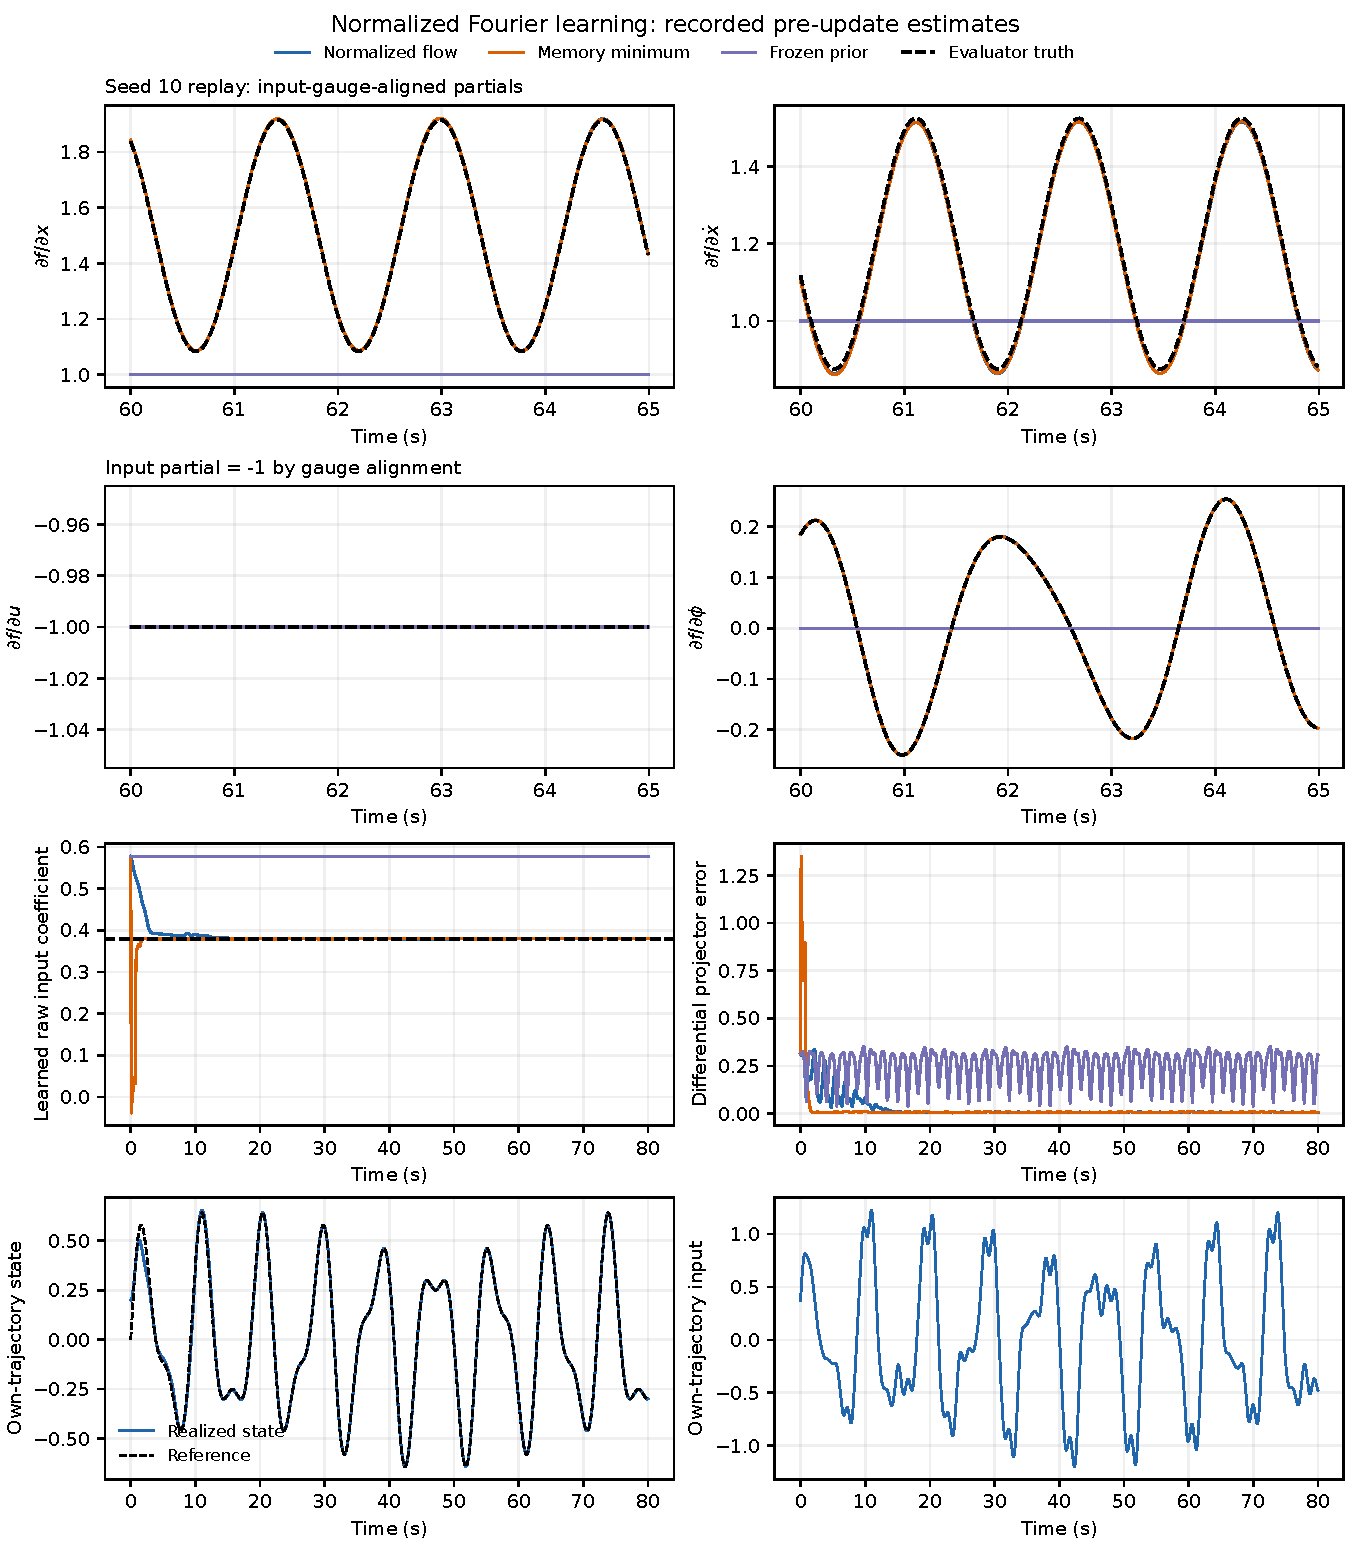
\includegraphics[width=.98\textwidth]{normalized_fourier_partials.pdf}
 \caption{Preselected seed-10 diagnostics, scored before assimilating the
 current secant. The upper four panels compare all three estimators on the
 replay stream over $60\le t<65$~s, a display window within the reporting
 interval.
 Estimates are divided by the learned input coefficient to use the physical
 reporting convention; dashed truth is evaluator-only. The input partial
 becomes $-1$ through this alignment, while all seven coefficients adapt.
 The middle panels show the raw input coefficient and differential projector
 error over the full episode, with every tenth sample displayed. The bottom
 panels alone show the normalized learner's own controlled state and input.
 The clock column includes both complete-product terms.}
 \label{fig:normalized_fourier_partials}
\end{figure*}

\begin{figure*}[t]
 \centering
 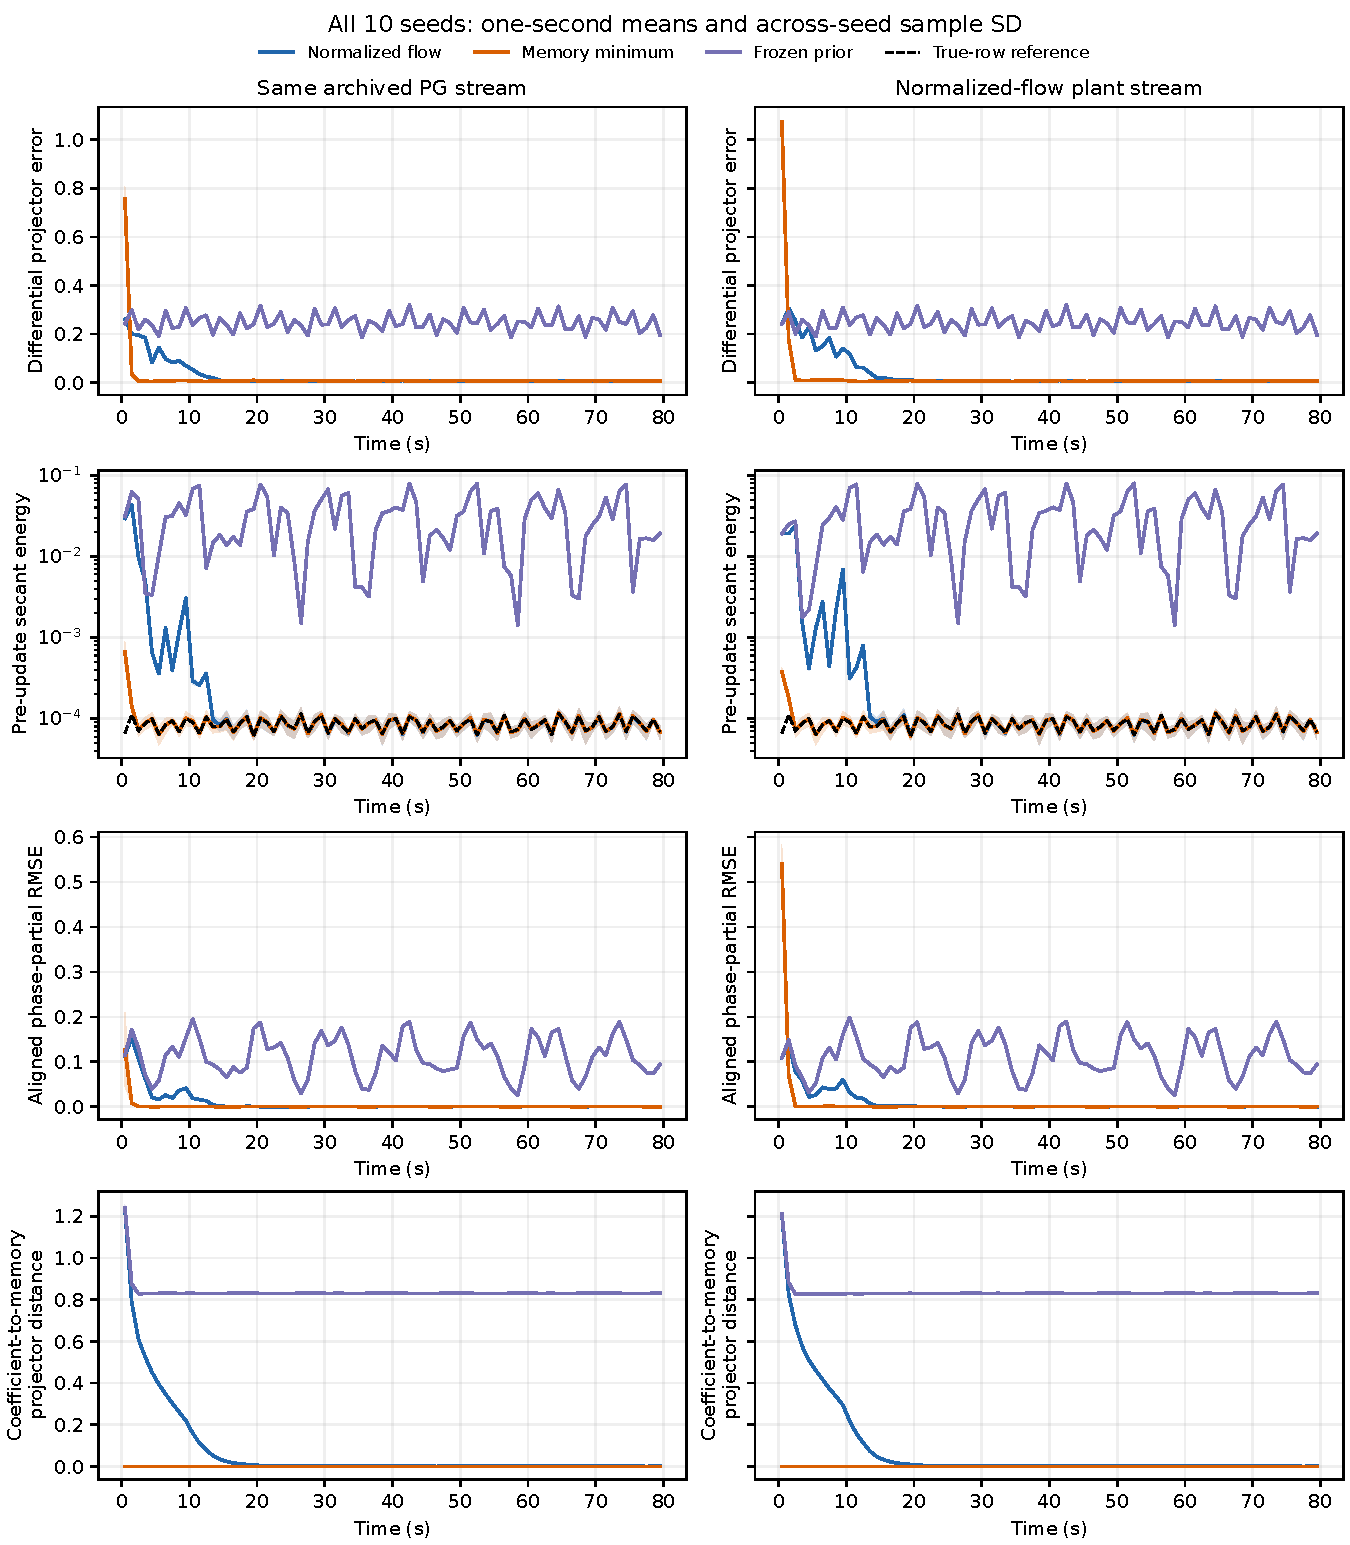
\includegraphics[width=.98\textwidth]{normalized_fourier_summary.pdf}
 \caption{Normalized-learning diagnostics for the replay and own-trajectory
 branches, each specifying ten seeds. Lines and shading show across-seed
 means and sample standard deviations after one-second nonoverlapping
 display aggregation; the phase-error panels use within-bin RMS. All table
 metrics use unsmoothed samples. Undefined startup energies and guarded
 shadow partials are omitted only from their display-bin averages and
 counted in the records; no reporting-window sample is missing. Comparators are same-stream
 bottom-eigenvector and frozen-prior shadows; their traces are not separate
 closed-loop control experiments. Coefficient normalization alone does not
 imply physical identification or successful control.}
 \label{fig:normalized_fourier_summary}
\end{figure*}

The implementation and declared protocol are
\path{experiments/normalized_fourier.py} and
\path{experiments/configs/normalized_fourier_20261118.json};
\path{docs/NORMALIZED_FOURIER_20261118.txt} explains the equations and replay
requirements. Run records contain observed channels, pre/post-update rows
and memories, solver counts, seeds, source/environment snapshots, replay-input
hashes, summaries, and failures, with partial traces retained on simulation
 failure. The executed audit and postprocessor are
 \path{experiments/audit_normalized_fourier.py} and
 \path{experiments/report_normalized_fourier.py}.
 Numerical flow refinement does not test a limit of the sensing period
 or secant window. The archive named in
\path{docs/NORMALIZED_FOURIER_20261118.json} is a local artifact outside
the repository, not a verified public download.

This retained historical demonstration and its diagnostics concern one
known integrable harmonic family
and calibrated readout. Low incompatibility, a positive noisy eigengap, or
accurate integration alone proves neither physical excitation nor closed-loop
stability. Its records are distinct from the earlier bounded comparison, and
it does not establish that the retained coefficient-based contact and Burgers
protocols implement the same normalized law.
